% mainfile: ../../../../master.tex
\subsection{Nucleic acid integrity assessment}
% The part of the label after the colon must match the file name. Otherwise,
% conditional compilation based on task labels does NOT work.
\label{task:20180321_cj0}
\tags{lab,dna,rna}
\authors{cj}
%\files{}
%\persons{}


\subsubsection{1\% Agarose gel preparation}

\begin{enumerate}
\item Measure with erlenmeyer 50~mL of 1\% agarose gel.\sidenote{The 1\% agarose gel is kept at 60\degree C in the gel room.}
\item Warm up the erlenmeyer for 15s in microwave: agarose will be more fluid and it will avoid bubbles when casting the gel
\item Cast the gel with the comb (for 15 wells)
\item Let the gel set for 20 min
\end{enumerate}

\comment{I cast my gel just after I arrived at work.}

\subsubsection{Sample preparation}

In a \gls{pcr} 8-well rack mix:
\begin{itemize}
\item For the DNA, I mix 6~\uL of DNA sample with 4~\uL of loading buffer (which is 15 ng of DNA)
\item For the RNA, I mix 2.5~\uL of RNA sample with 7.5~\uL of loading buffer (which is 100 ng of RNA)
\item Tap gently pipette mix
\end{itemize}

\subsubsection{Electrophoresis}

For this electrophoresis migration, we run:
\begin{itemize}
\item 10~\textmu L of each sample 
\item 5~\textmu L of the 1~kb ladder
\item 5~\textmu L of the 2-log ladder
\end{itemize}
\comment{I leave empty lanes between ladders and samples.}

\begin{enumerate}
\item Place the agarose gel into the gel box (electrophoresis unit) containing TAE buffer
\item Load 5~\textmu L of molecular weight ladder into the first and last lane of the gel
\item Load 9~\textmu L of each sample into the additional wells of the gel
\item Run for 60 min with the \gls{eps} 301 at 80~V, 400~mA
\item Remove gel from the migration tank and place in the staining container (a recycled tip box).
\end{enumerate}

\subsubsection{SYBR\cR Gold Staining}

\begin{enumerate}
\item Ensure SYBR\cR gold is properly thawed.
\item Ensure the pH of \gls{tae} buffer is between 7.5 and 8
\item Prepare the staining solution at 1X SYBR\cR Gold in \gls{tae} buffer.
\item Transfer 100 mL of staining solution in the staining container.
\item Incubate under agitation for 30 min.
\item Visualize your nucleic acid fragments with \gls{uv} lights.
\end{enumerate}
\comment{The \gls{ccd} camera by BioRad does not work anymore. In the meanwhile, we use transilluminator and take the picture with my cell phone.}

\subsubsection{Results}

\begin{figure}[H] % position of the figure 
    \centering
    \caption{Picture of the gel after migration}
   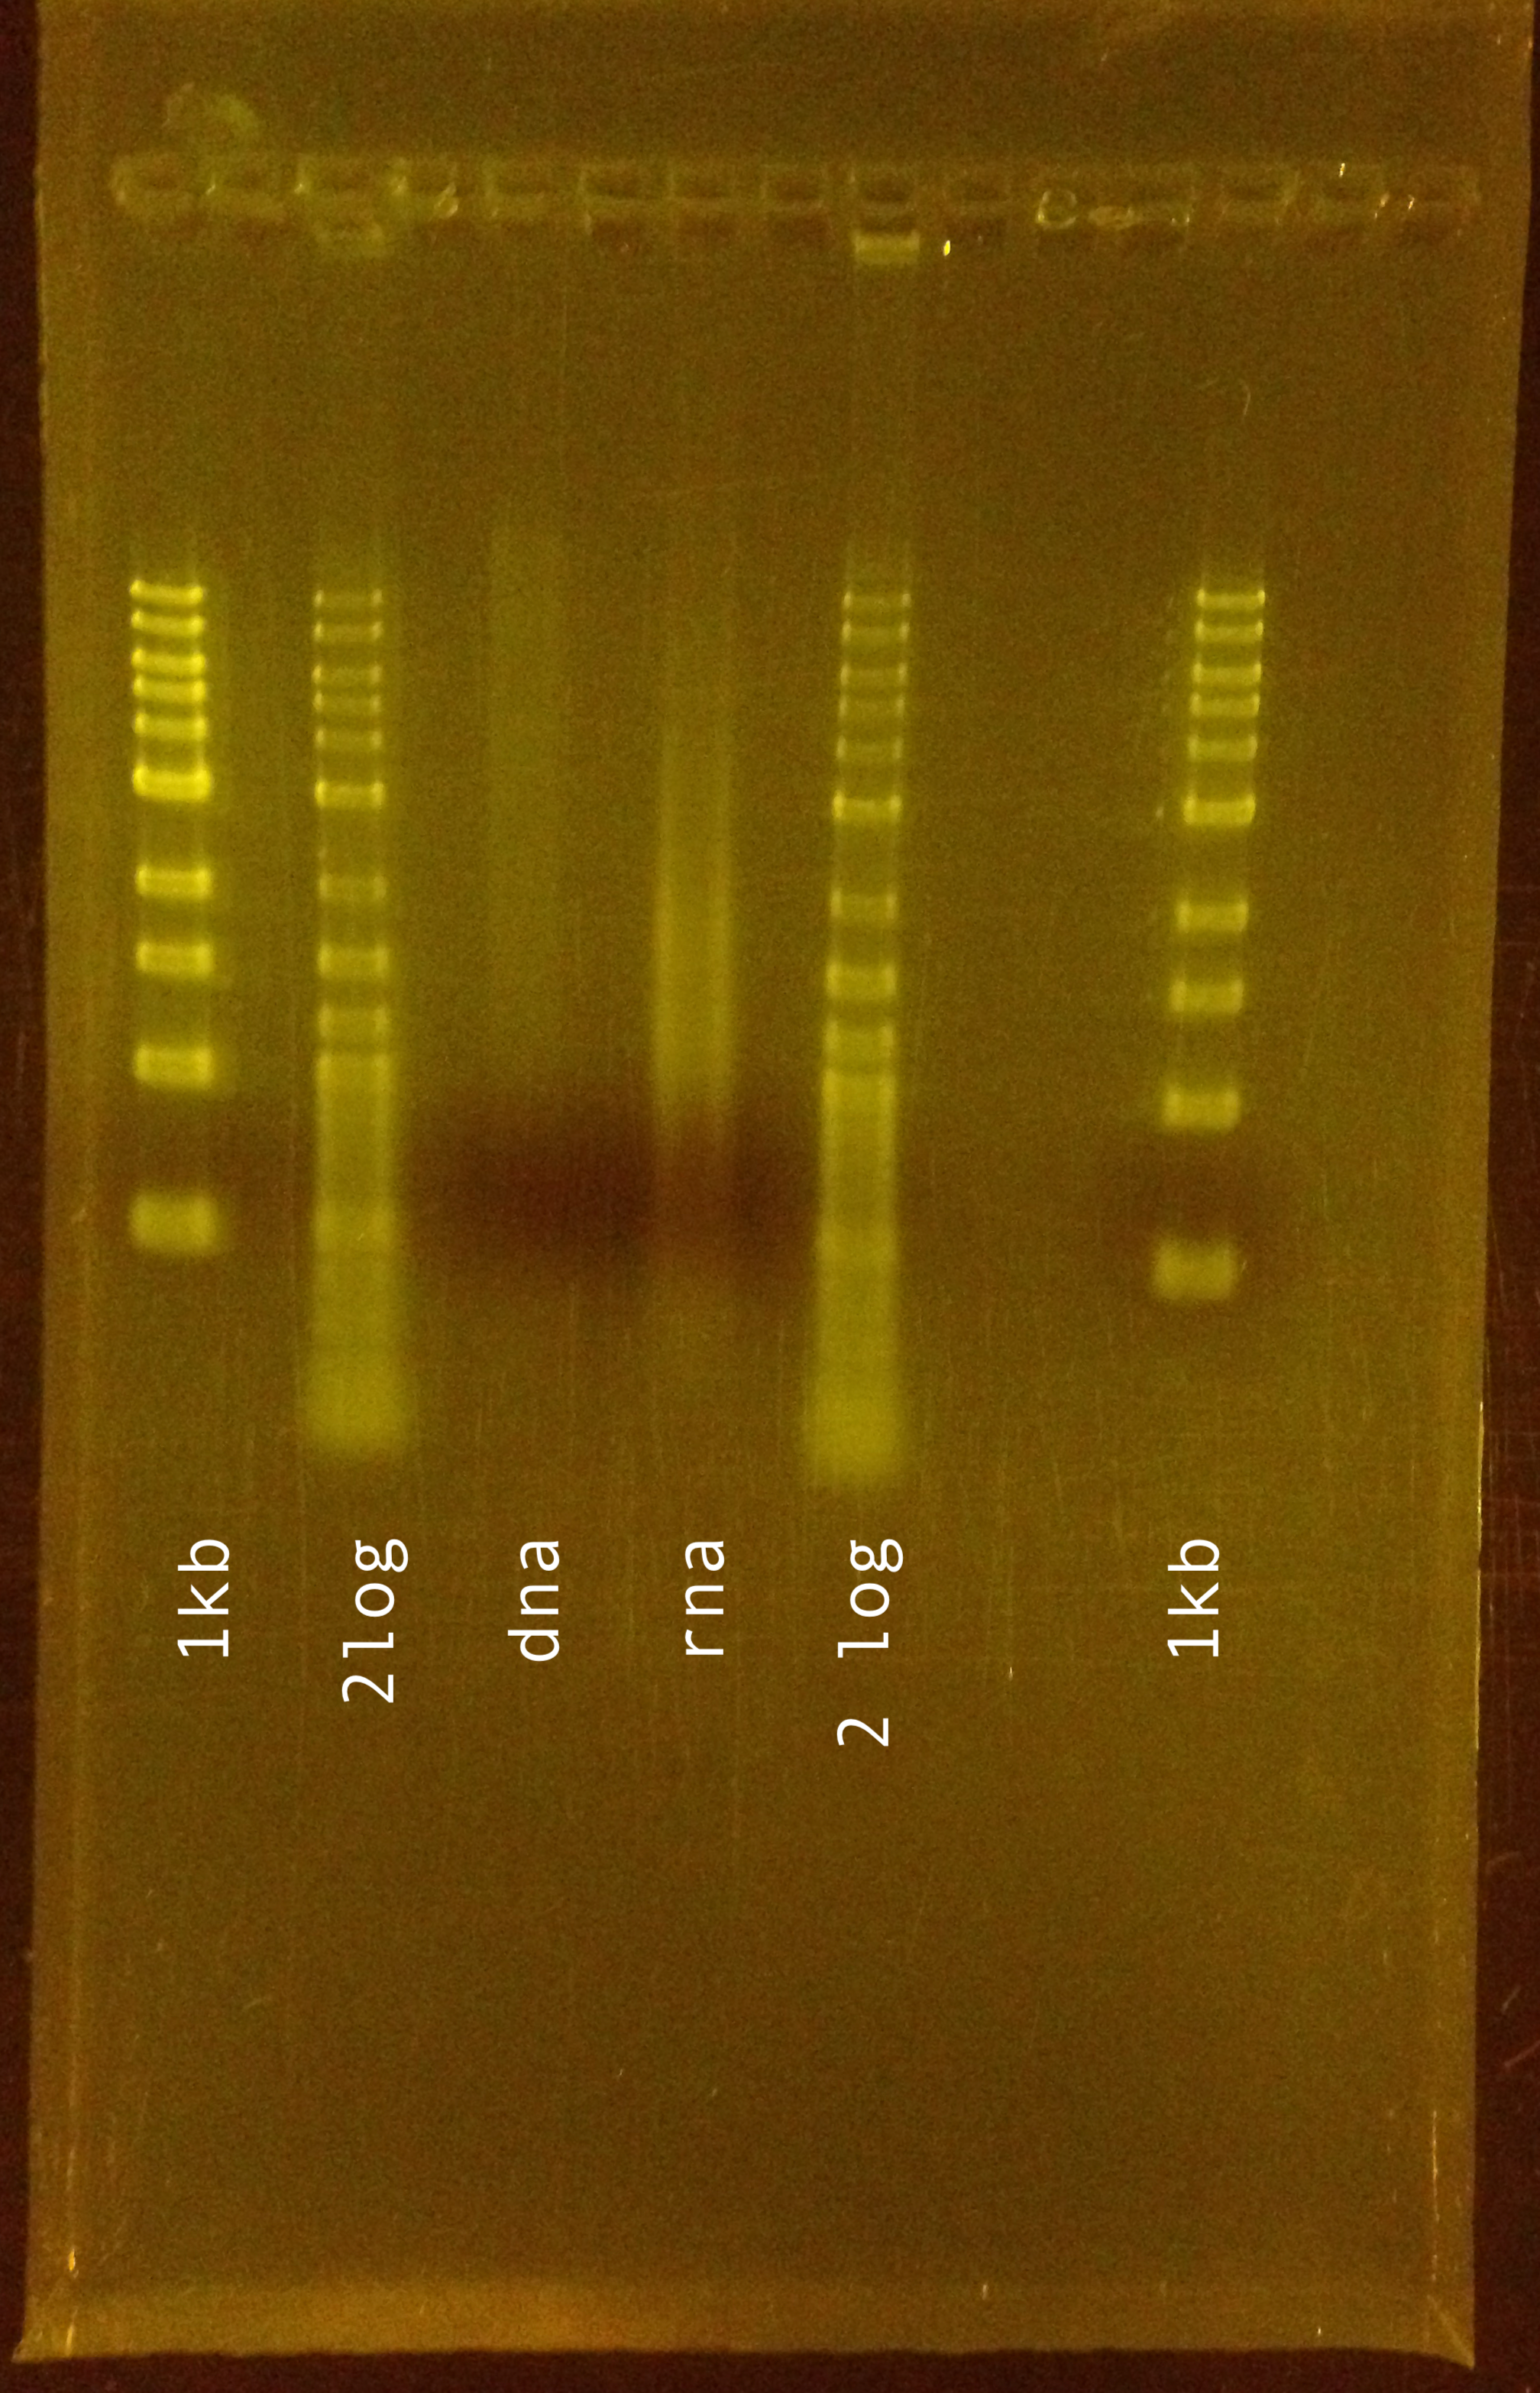
\includegraphics[width=0.5\textwidth]{graphics/pic/20180320_gel_sybr_gold.png}
\end{figure}\sidenote{\url{https://www.researchgate.net/post/Can_anyone_help_me_with_gel_electrophoresis_of_total_RNA}}

Compared to the previous gels I obtained with SYBR\cR Gold, the genomic DNA does not show a clean band. This can be explained by the fact that I was working with cultures before which means one size of genomic DNA was very abundant compared to others while this DNA was obtained from a Sterivex\texttrademark~ filter containing a variety of species. Same thing can explain the fact that the rRNA bands seems a lot more blurry than previously. 

\subsubsection{Discussion}

After quick search on the internet, the fact that I am unable to identity specific bands for the RNA sample makes sense. For \textit{E.coli}, the 16S rRNA molecule is 1.5 kb and the 23S rRNA molecule weights 2.9~kb. For yeast, the 18S rRNA molecule is 2.0 kb and the 26S rRNA molecule weights 3.8~kb. And there are also more smaller RNA molecules like \gls{mrna} and \gls{trna} (and maybe miRNA?). So with rRNA molecules from a wide variety of orgsnisms, it is not surprising to observe a long smearing lane. Also, it is important to keep in mind that this gel does not allow me to determine the sizes of the RNA molecules because RNA will not run on agarose gel exactly according to it's size: the migration of RNA molecules will be affected by the secondary and tertiary structures of the RNA molecules. Therefore, it is necessary to use denaturing gel (formaldehyde, urea, methyl mercury, etc.) and compare it to a RNA ladder!

